\chapter{Implementierung}

\section{Entwicklungsumgebung für WebXR und Oculus Quest 3}

Die Entwicklung von WebXR-Anwendungen für die Oculus Quest 3 erfordert eine spezielle Entwicklungsumgebung für einen effizienten Entwicklungsprozess.
Dabei müssen verschiedene Technologien und Tools miteinander kombiniert werden, um eine reibungslose Entwicklung und ein möglichst schnelles Testen der Anwendung zu ermöglichen.

Der erste Schritt ist das Anzeigen der WebXR-Anwendung auf der Oculus Quest 3.
Das Problem dabei im Vergleich zu \glqq{}normalen\grqq{} Webanwendungen ist, dass WebXR-Anwendungen nur über HTTPS aufgerufen werden können.
Das bedeutet, dass die Anwendung über HTTPS gehostet werden muss, um direkt vom Browser der Oculus Quest 3 aufgerufen werden zu können.
Hierfür gibt es verschiedene Möglichkeiten, wie beispielsweise das Erstellen eines eigenen Zertifikats für den lokalen Entwicklungsrechner oder das Hosting der Anwendung auf einem Server mit HTTPS-Unterstützung.
Für den Rahmen der Entwicklung dieser Bachelorarbeit wird die Anwendung jedoch, wie auch in der Artikelserie des Taikonautenmagazins \autocite[Part 0/8]{taikonauten-magazine} empfohlen, mit LocalTunnel gehostet, um die Anwendung direkt von der Oculus Quest 3 aus testen zu können.
LocalTunnel erstellt einen temporären HTTPS-Link, über den die Anwendung aufgerufen werden kann, ohne dass ein eigenes Zertifikat oder ein eigener Server notwendig ist.
Dafür muss die Anwendung nur lokal auf dem Entwicklungsrechner laufen und der LocalTunnel-Client gestartet sein, um den temporären Link zu generieren.
Als zusätzliche Sicherheit muss dann beim Aufrufen der Seite noch die IP-Adresse des Entwicklungsrechners angegeben werden, um sicherzustellen, dass nur der Entwickler die Anwendung testen kann.
Dies muss in der Regel jedoch nur einmal nach jedem Neustart oder Crash gemacht werden, da der Link für die Dauer der Sitzung gespeichert wird.

Der nächste Schritt, wenn Zugriff mit der Oculus Quest 3 auf die WebXR-Anwendung besteht, ist die Anzeige von Entwickler-Tools und Debugging-Informationen der Oculus Quest 3.
Da die Oculus Quest 3 auf Android basiert, kann auf dem Entwicklungsrechner Android Debug Bridge (ADB) installiert werden, um über USB eine Verbindung zur Oculus Quest 3 herzustellen.
Die Verbindung muss noch in der VR-Brille bestätigt werden, um den Zugriff auf die Entwickleroptionen zu ermöglichen.
Ist das geschehen, erscheint die Quest 3 mit ihren geöffneten Websites in der Geräteliste der Chrome DevTools, die über die URL \url{chrome://inspect/#devices} aufgerufen werden können.
Dort können dann die Entwickler-Tools der Oculus Quest 3 geöffnet werden, um beispielsweise die Performance der Anwendung zu überwachen und Fehlermeldungen zu sehen.


Für viele Aspekte der Entwicklung von XR-Anwendungen, wie beispielsweise einfache Tests von Interaktionen wie einzelnen Klicks können auch über einen WebXR-Emulator direkt am Entwicklungsrechner getestet werden.
In dieser Arbeit wird dafür die Chrome-Erweiterung Immersive Web Emulator von Meta verwendet, die es ermöglicht, WebXR-Anwendungen direkt im Browser zu testen.
Mit dieser Erweiterung wird für WebXR ein einfacher Raum mit einem Headset und den beiden Meta Quest Controllern simuliert.
Das Headset sowie die beiden Controller können unabhängig voneinander über die Erweiterung positioniert und gesteuert werden.
In dem in Abbildung \ref{fig:webxr-emulator} links dargestellten Panel können verschiedene Interaktionen, wie beispielsweise Klicks oder das Bewegen der Controller, simuliert werden, um die Anwendung zu testen.
Der Emulator generiert dann eine live Vorschau der Anwendung, die direkt im Browser angezeigt wird.

\begin{figure}[H]
    \centering
    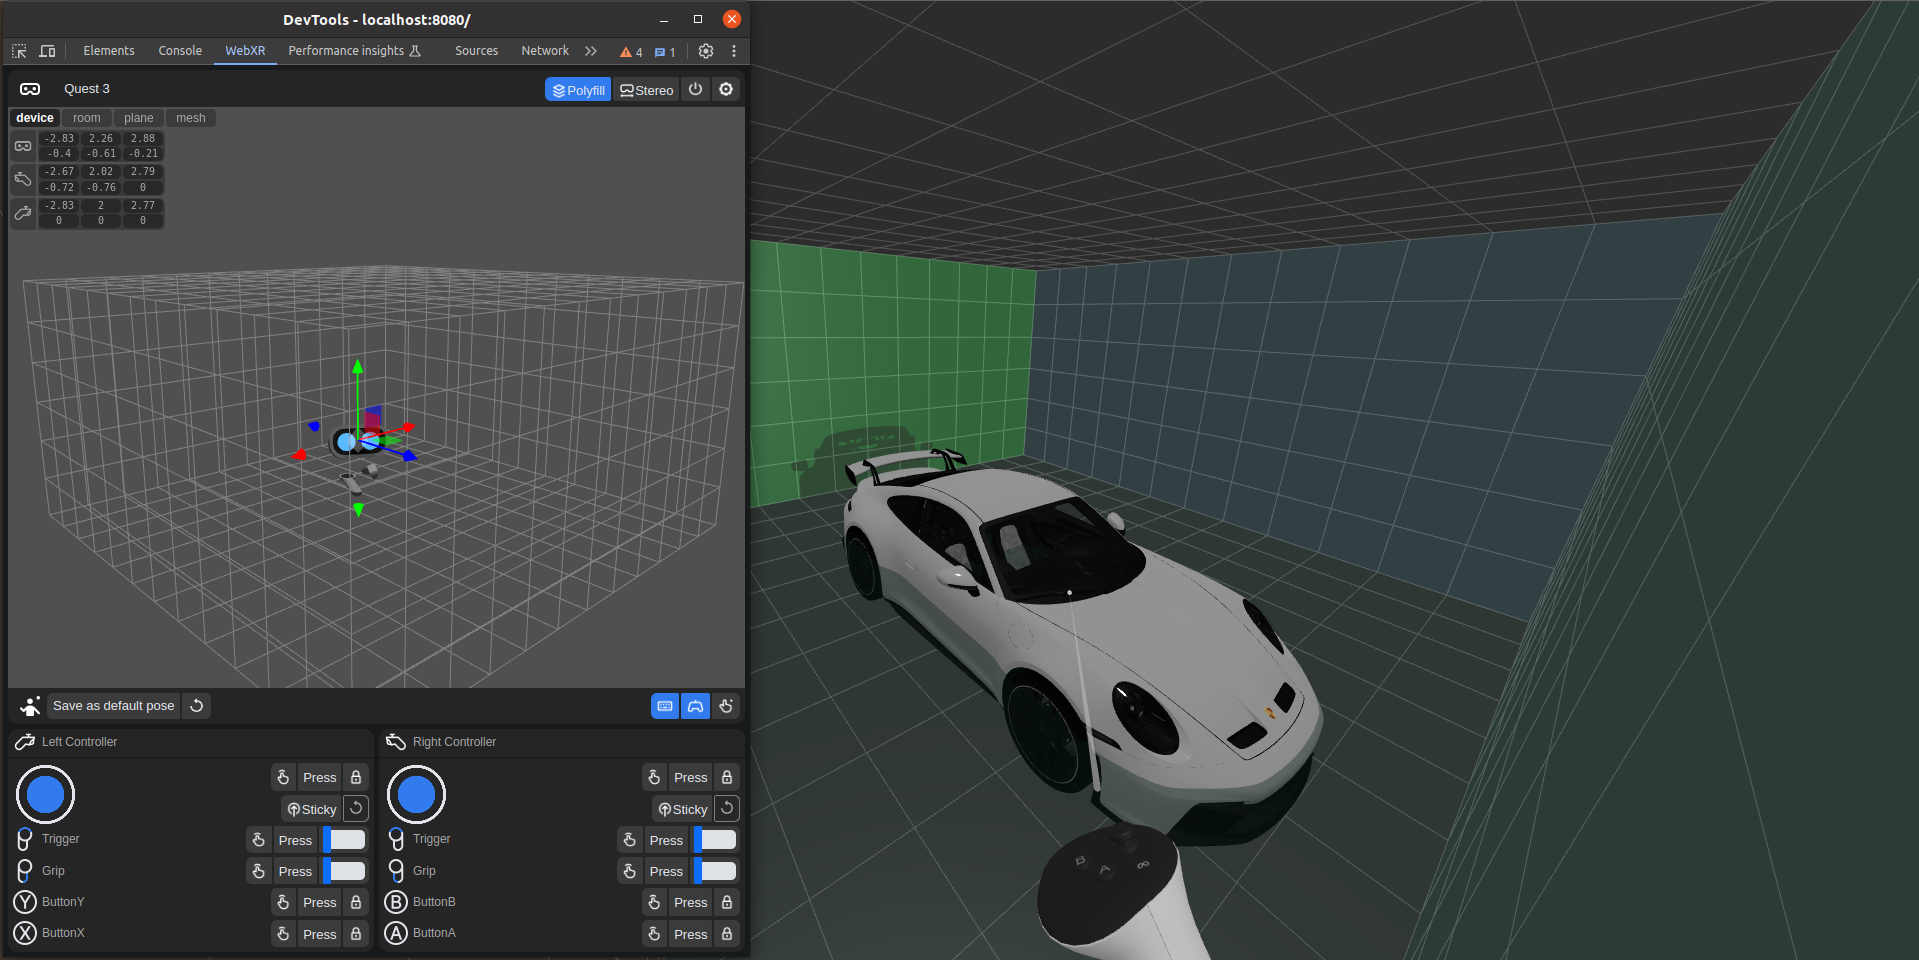
\includegraphics[width=0.8\textwidth]{images/WebXR-Emulator.png}
    \caption{Screenshots der Immersive Web Emulator Erweiterung in Chrome}
    \label{fig:webxr-emulator}
\end{figure}

Das Testen der Anwendung mit dieser Erweiterung ist deutlich schneller und einfacher als das Testen auf der Oculus Quest 3, da die Anwendung direkt im Browser getestet werden kann und keine Verbindung zur Oculus Quest 3 notwendig ist.
Zudem sind die Ladezeiten beim Neuladen der Anwendung deutlich kürzer, da die Anwendung nicht auf die Übertragung der Daten auf die Oculus Quest 3 warten muss.
Dennoch ist es wichtig, die Anwendung auch regelmäßig auf der Oculus Quest 3 zu testen, da die Performance und die Interaktionen auf dem Emulator nicht immer exakt der Realität entsprechen.



\section{Implementierung der Anwendung}

In diesem Kapitel wird der Prozess der Implementierung der Anwendung beschrieben.
Dabei wird zunächst die Entwicklung der grundlegenden zu implementierenden Konzepte beschrieben, bevor auf die tatsächliche Implementierung der ausgearbeiteten Interaktionskonzepte eingegangen wird.

\subsection{Interaktionskonzepte für Requirements}

Die Bachelorarbeit beschäftigt sich mit der Darstellung von Requirements in AR beziehungsweise VR.
Dabei soll untersucht werden, wie Anforderungen in einer 3D-Umgebung dargestellt werden könnten.
Dazu werden verschiedene Interaktionskonzepte entwickelt, welche als Basis für die Implementierung mit WebXR dienen.


\subsubsection{Beispiel 1: Explodierende Bauteile}

Das erste untersuchte Interaktionskonzept ist hauptsächlich für die Darstellung von Anforderungen von Produkten gedacht.
Die Idee ist, ein Produkt in einer Animation in seine einzelnen Bauteile zu zerlegen und die Anforderungen auf ihren zugehörigen Bauteilen darzustellen.
In der Animation werden die Bauteile von einem Punkt in der Mitte des Produkts nach außen bewegt, sodass sie sich um den Ursprungspunkt des Produkts herum anordnen.
Beispielsweise könnte ein Auto so zerlegt werden, dass bei der Animation die Räder, die Karosserie, der Motor und die Innenausstattung einzeln als eigene Objekte sichtbar werden.
So kann der Nutzer das gesamte Produkt betrachten und sich dann auf Wunsch einzelne Bauteile und deren Anforderungen genauer ansehen.

Die Anforderungen sollen dabei als Text auf UI-Panelen dargestellt werden, die an den zugehörigen Bauteilen angebracht sind.

Am bereits genannten Beispiel des Autos wird klar, dass die Komplexität der Darstellung bei vielen Bauteilen schnell ansteigt und die Übersichtlichkeit verloren gehen kann.
Daher ist es bei umfangreichen Produkten eventuell sinnvoll, die Darstellung der Bauteile in mehreren Schritten zu realisieren.
Zum Beispiel könnte in einer Übersicht das gesamte Auto in wenigen Bauteilen dargestellt werden, indem beispielsweise ein Rad, das eigentlich aus Reifen, Felge, Radmuttern, Bremsscheibe etc. besteht, als ein einzelnes Objekt dargestellt wird.
Will der Nutzer dann die Räder genauer betrachten, kann er in eine Detailansicht wechseln, in der nur ein Rad mit all seinen Bauteilen animiert wird.
So lässt sich eine hohe Komplexität der Darstellung erreichen, ohne dass die Übersichtlichkeit verloren geht.


Für diese Darstellung soll der Nutzer zunächst mithilfe eines Controllers einen Ort für die Darstellung im Raum auswählen.
Dieser Ort wird als Ursprungspunkt für die Darstellung der Bauteile verwendet.
Dann soll der Nutzer frei durch die Explosionsanimation navigieren können, um sich die Bauteile aus verschiedenen Perspektiven anzusehen.

Auch bei Software-Requirements ist es denkbar, diese in ihre Komponenten zu zerlegen und zu diesen Komponenten zugehörige Anforderungen darzustellen.
Jedoch bietet die Darstellung in AR bzw. VR hierbei quasi keine Vorteile im Gegensatz zu einer 2D-Darstellung auf einem Bildschirm.
Bei Software-Anwendungen ist die einfache Darstellung auf einem Bildschirm näher an der tatsächlichen Laufumgebung der meisten Softwares als bei physischen Produkten, bei denen durch eine dreidimensionale Darstellung ein Mehrwert entstehen kann.

Bei diesem Konzept soll die Realisierbarkeit solcher Darstellungen für physische Produkte untersucht werden.
Dabei muss die Kosten-Nutzen-Relation kritisch betrachtet werden, da die Implementierung einer solchen Darstellung sehr aufwändig sein kann und daher einen hohen Mehrwert gegenüber anderer Darstellungen bieten muss.

\subsubsection{Beispiel 2: Wolken von Anforderungen}

Der Ansatz der explodierenden Bauteile ist aufgrund der Individualität des Konzepts sehr zeitaufwendig und komplex zu implementieren.
Zudem ist dieser Ansatz nur für die Darstellung von Produkten, also physischen Systemen, geeignet.
Daher wird ein weiteres Interaktionskonzept entwickelt, welches sich theoretisch auch automatisiert generieren lässt und für alle Arten von Anforderungen geeignet ist.

Die grundlegende Idee ist, Anforderungen in Wolken von Texten darzustellen, also als eine Gruppierung von UI-Elementen im Raum.
Hierbei soll eine räumliche Gruppierung der Anforderungen nach verschiedenen Kriterien möglich sein.
Beispielsweise könnten Anforderungen, die zu einem bestimmten Feature gehören, in einer Wolke gruppiert werden, während Anforderungen, die zu einem anderen Feature gehören, in einer anderen Wolke gruppiert werden.
Durch die räumliche Anordnung der Wolken kann der Nutzer schnell erkennen, welche Anforderungen zusammen gehören und welche nicht.

Dabei soll es auch möglich sein in Wolken hinein- und herauszuzoomen, um die Granularität der angezeigten Anforderungen zu erhöhen.
Gehen wir dabei wieder vom Beispiel des Autos aus, könnte es möglich sein in die Wolke der Räder hineinzuzoomen, um die Anforderungen an die Reifen, Felgen, Radmuttern etc. zu sehen.
Daraufhin kann wieder herausgezoomt werden, um die Anforderungen an das gesamte Auto zu sehen.
Eine weitere Möglichkeit wäre es, auf den Anforungspanels Filtermöglichkeiten für verschiedene Beziehungen der Anforderung darszustellen, um dann bei einer Auswahl in die neue Anforderungswolke zu zoomen.
Diese Interaktion und die räumliche Anordnung der Wolken sollen dem Nutzer helfen, auch bei einer großen Anzahl von Anforderungen einen Überblick zu behalten und schnell die gewünschten Anforderungen zu finden.

Bei diesem Konzept soll vor allem der Vorteil gegenüber einer 2D-Darstellung kritisch untersucht werden.
Denn die Darstellung der Anforderungen in Wolken ist prinzipiell auch in 2D möglich, auch mit der Interaktionsmöglichkeit des Hinein- und Herauszoomens.
Daher soll untersucht werden, ob die räumliche Anordnung der Anforderungen in AR tatsächlich einen Mehrwert gegenüber einer 2D-Darstellung bietet und ob die Interaktionen intuitiv und effizient sind.


\subsubsection{Beispiel 3: Anforderungen als 3D-Objekte}

\subsection{Implementierung der Interaktionskonzepte}

In den folgenden Abschnitten wird auf die Implementierung der zuvor beschriebenen Interaktionskonzepte eingegangen.
Dabei werden grundlegende Konzepte und Technologien vorgestellt und erklärt, die für die Implementierung notwendig sind.
Zudem werden Screenshots der implementierten Konzepte gezeigt und die Funktionsweise der Interaktionen beschrieben.
Dabei werden auch die Herausforderungen und Probleme bei der Implementierung aufgezeigt und diskutiert.

Vor der Implementierung des Konzepts muss zunächst eine grundlegende WebXR-Anwendung erstellt werden, die die Interaktionen mit dem Controller ermöglicht.
Hierfür wird das Skelett einer WebXR-Anwendung aus einer Artikelserie des Taikonauten-Magazins verwendet, welches als Basis für die Implementierung dient \autocite[][]{taikonauten-magazine}.
Die Anwendung nutzt bereits die vom Nutzer gescannten Umgebungen, um einen virtuellen Raum zu erstellen, in dem die Interaktionen stattfinden.
Dabei werden Wände und Böden der Umgebung erkannt und als Mesh in die Szene eingefügt, um dem Nutzer eine Interaktion mit der realen Umgebung zu ermöglichen.
Zudem wurden schon einige Interaktionen des Controllers, wie das Auswählen von Objekten durch Raycasting, implementiert, die als Basis für die Implementierung der Interaktionskonzepte dienen.



\subsubsection{Explodierende Bauteile}

Der erste Schritt bei der Implementierung des Interaktionskonzepts der \glqq{}explodierenden\grqq{} Bauteile ist die Erstellung eines 3D-Modells, welches die Bauteile des Produkts enthält.
Dabei muss jedes Bauteil als eigenes Objekt im 3D-Modell vorhanden sein, um sie in der Animation separat darstellen und referenzieren zu können.
Für die erste Implementierung wird ein einfaches 3D-Modell eines Tetris Blocks verwendet, welcher aus 4 verschiedenfarbigen Bauteilen besteht.

Dieses Modell wurde in Blender erstellt und als 3D-Modell im glTF-Format, welches wie WebXR von der Khronos Group entwickelt wurde, in die Anwendung exportiert.
Das glTF-Format ist ein offenes 3D-Dateiformat, welches für die effiziente Übertragung von 3D-Modellen im Web optimiert ist und die Dateigröße möglichst klein hält.
Ein weiterer Vorteil des glTF-Formats ist, dass es auch Animationen und Materialien unterstützt, die im 3D-Modell enthalten sind.
So kann die Animation der Bauteile auch direkt in der Modellierungssoftware erstellt und in das glTF-Modell mit eingebacken werden.

Der nächste Schritt ist das Platzieren des erstellten 3D-Modells in der WebXR-Umgebung.
Dazu wird das Prinzip des Raycastings verwendet, um dem Nutzer zu ermöglichen, mit dem Controller einen Punkt im Raum auszuwählen, an dem das 3D-Modell platziert werden soll.
Der Raum, in dem sich der Anwender befindet, muss dafür zu Beginn einmalig in den Meta Quest Einstellungen eingescannt werden.
Ist das geschehen, werden durch das Skelett der Anwendung des Taikonauten-Magazins bereits die Wände und Böden der Umgebung als Meshes erkannt und in die Szene eingefügt.
Dann wird vom Controller ein Strahl in die Szene geschossen, und der Punkt, an dem der Strahl ein Objekt trifft, wird als Event zurückgegeben.

An diesem Punkt wird dann ein Ankerpunkt erstellt, an den das 3D-Modell angehaftet wird.
Dieser Ankerpunkt ist ein Babylon.js-Objekt, welches einen Punkt im Raum in AR an einer bestimmten Position darstellen kann.
Das 3D-Modell wird dann an diesen Ankerpunkt angehängt, sodass es sich relativ zu diesem Punkt bewegt.


Ist das 3D-Modell platziert, kann die Animation des Produkts gestartet werden.
Dafür wird ein Knopf des Controllers als Start-Button für die Animation verwendet, mit dem sich die Animation vorwärts und wieder rückwärts abspielen lässt.
Für die Animation wird die aus Blender in das glTF-Modell eingebackene Animation verwendet.
Dafür wird in Babylon.js eine Animationsfunktion erstellt, die die Animation des Modells über einige Parameter, wie beispielsweise den Start- und Endframe der Animation, steuert.
So kann für die Vorwärts- und Rückwärtsanimation die gleiche Funktion verwendet werden, indem die Start- und Endframe-Parameter basierend auf einem globalen Boolean, der den Animationsstatus speichert, gesetzt werden.

Beim Abspielen der Animation wird jedes Bauteil des Produkts in einer Schleife durchgegangen und dessen Animation gestartet.
Diese Schleife wird dann auch genutzt, um den einzelnen Bauteilen ihre Anforderungen als Text-UI-Elemente zuzuweisen.
Dafür wird in Babylon.js eine Fläche erstellt, auf der der Text dargestellt wird, und diese Fläche an das Bauteil angehängt.
Die Fläche kann dabei auch als Knopf funktionieren, um bei einem Klick beispielsweise das Bauteil zu vergrößern.
Diese UI-Elemente werden aber, wie in Abbildung \ref{fig:tetris-explosion} zu sehen ist, nur angezeigt, wenn das Produkt gerade \glqq{}explodiert\grqq{} ist und nicht, wenn das Produkt gerade im Normalzustand ist.

\begin{figure}[H]
    \centering
    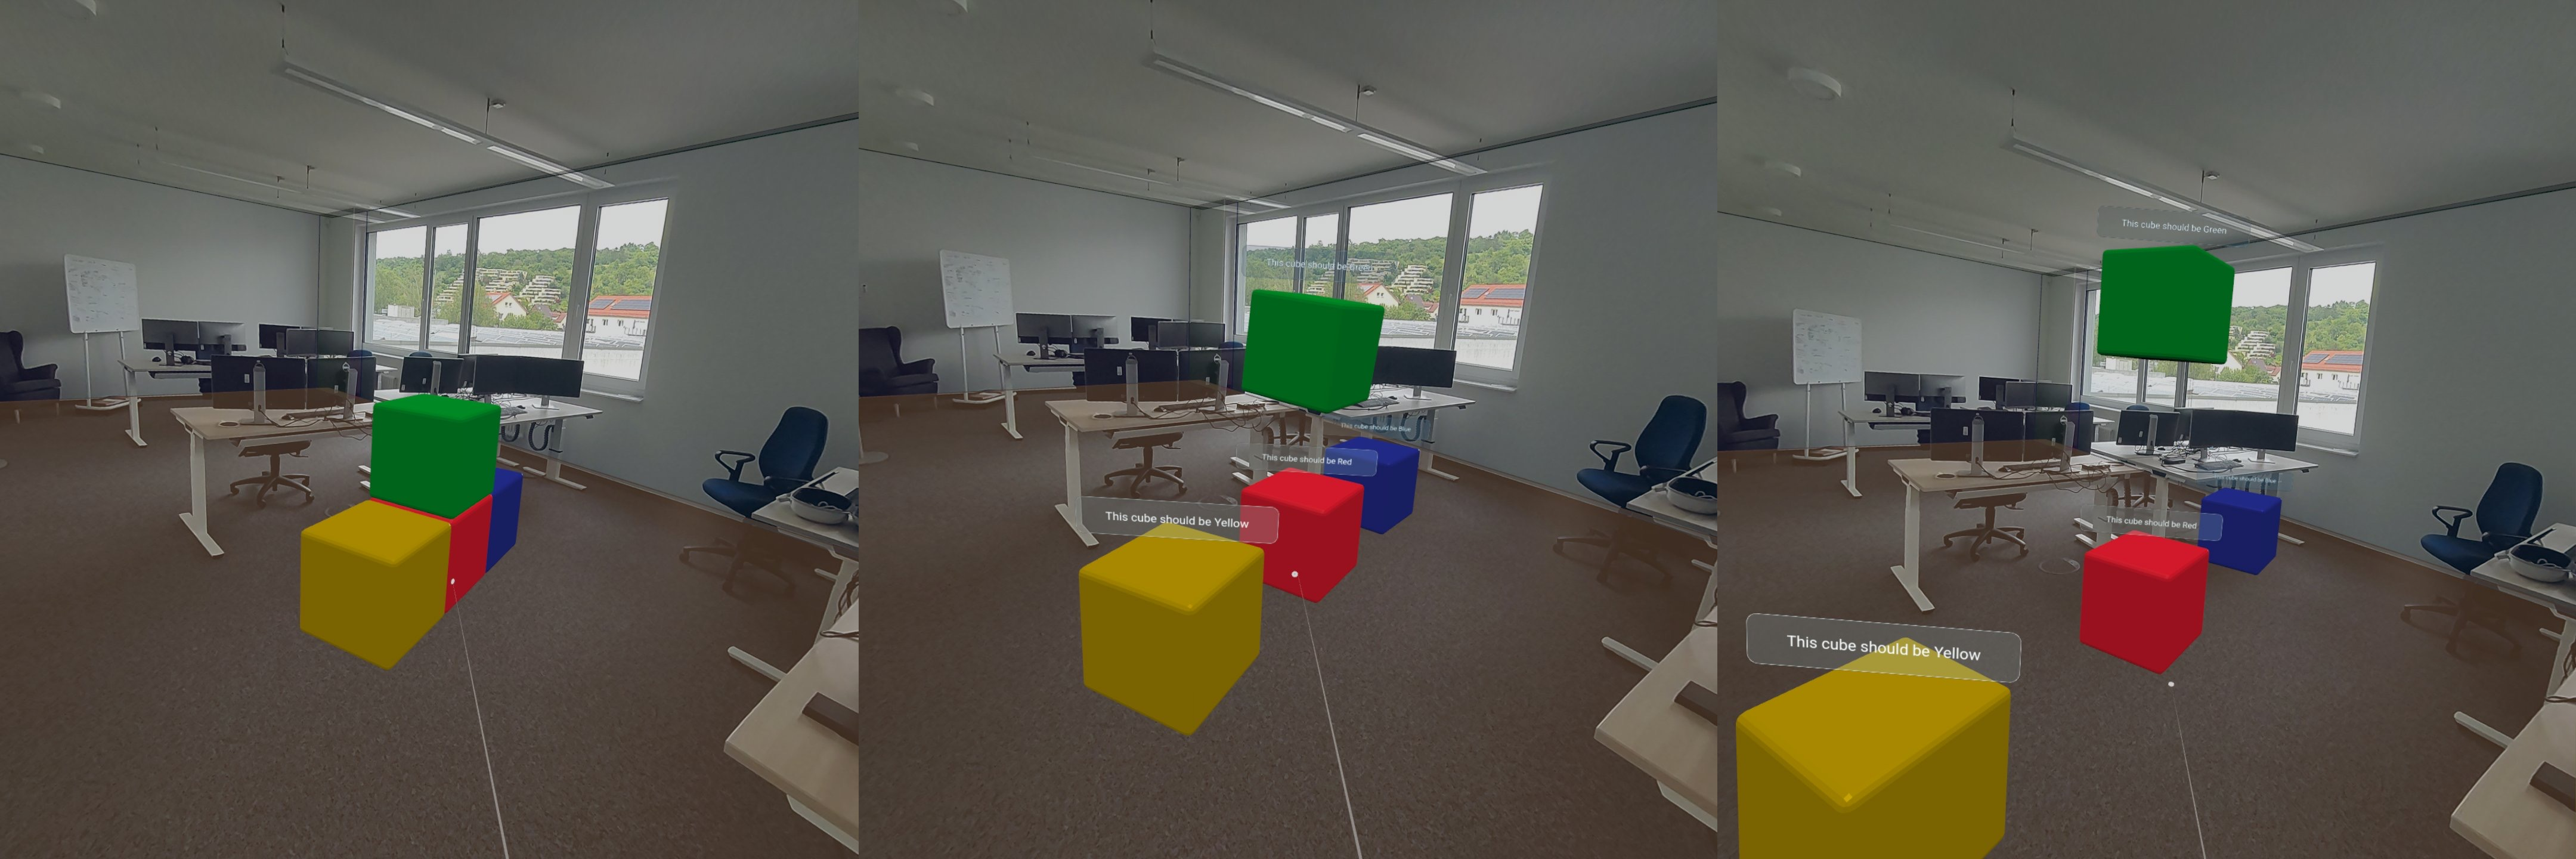
\includegraphics[width=1\textwidth]{images/tetris-explosion.png}
    \caption{Screenshots des explodierenden Tetris-Blocks mit Anforderungen in AR}
    \label{fig:tetris-explosion}
\end{figure}

\subsubsection{Implementation an einem komplexeren Modell}

Nachdem das Interaktionskonzept funktionell am einfachen Modell eines Tetris-Blocks implementiert wurde, ist die nächste Herausforderung die Implementierung an einem komplexeren Modell.
Dafür wird ein relativ detailliertes 3D-Modell eines Porsche 911 von der 3D-Asset-Website Sketchfab verwendet, welches von dem Nutzer Abdul Azim Sharif erstellt und unter der CC BY 4.0 Lizenz veröffentlicht wurde \autocite[][]{SketchfabPorsche}.
Das Modell, welches in Abbildung \ref{fig:porsche} zu sehen ist, wurde ausgewählt, da es viele verschiedene Bauteile enthält, die in der Animation separat dargestellt werden können.

\begin{figure}[H]
    \centering
    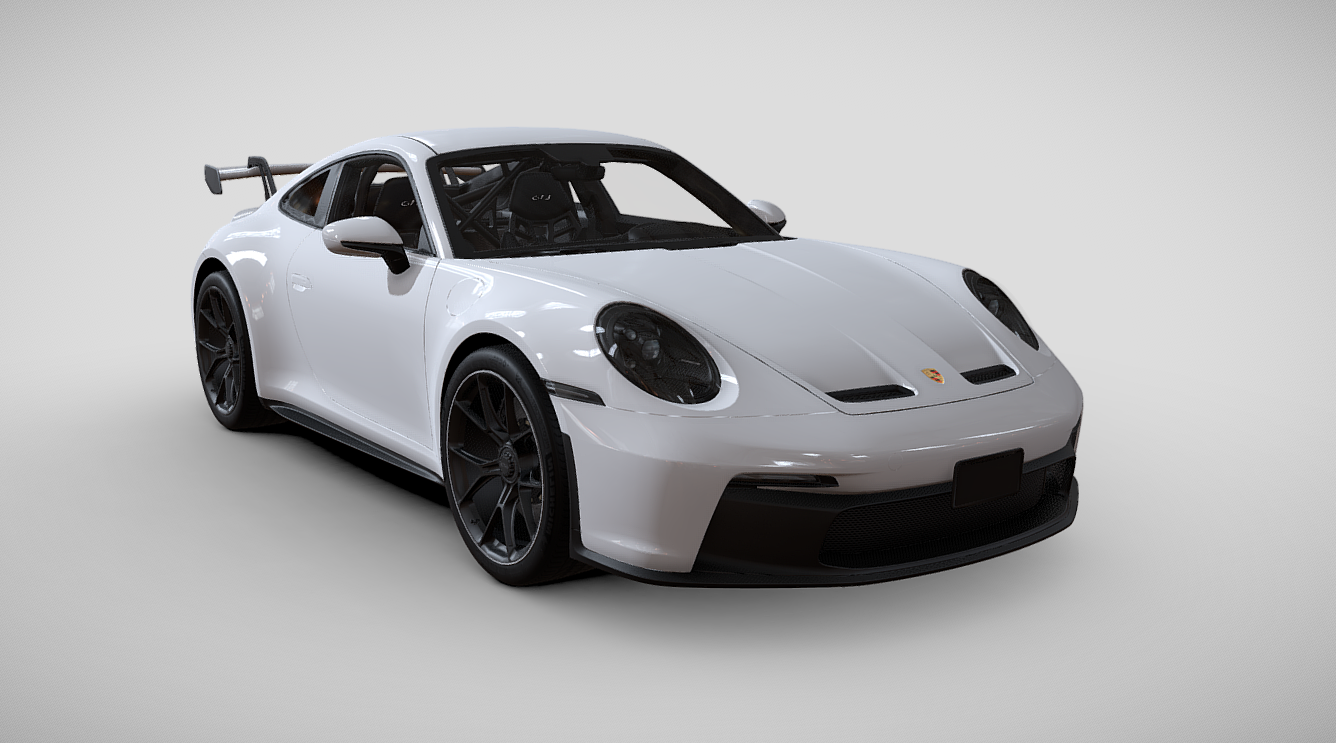
\includegraphics[width=0.7\textwidth]{images/PorscheModell.png}
    \caption{Screenshot des in der Anwendung genutzten Porsche Modells}
    \label{fig:porsche}
\end{figure}

Bei dem in dieser Bachelorarbeit verwendetem Modell ist es jedoch wichtig zu beachten, dass es sich um kein vollständig akkurates und funktionales Modell eines Autos handelt.
Beispielsweise existieren keine Achsen an denen die Räder hängen.
Für den anschaulichen Zweck dieser Bachelorarbeit ist das Modell jedoch ausreichend, da es genug \glqq{}reale\grqq{}  Bauteile enthält um das Interaktionskonzept zu demonstrieren.
Würde das Interaktionskonzept in einer echten Anwendung für Kunden verwendet werden, sollte jedoch mit möglichst akkuraten CAD-Modellen gearbeitet werden, um die Anforderungen an die Bauteile möglichst genau darzustellen.
Auf die Möglichkeit einer solchen professionellen Anwendung wird in der Diskussion eingegangen.

Für die Verwendung des Modells in der Anwendung muss als nächstes eine Animation mit dem Modell erstellt werden, die die Bauteile des Autos in ihre Einzelteile zerlegt.
Dafür wird in Blender eine Animation erstellt, welche einige Bauteile, wie beispielsweise die Verkleidung, die Räder und der Spoiler, nach außen weg bewegt.
Zum besseren Verständnis ist in Abbildung \ref{fig:porsche-explosion} eine Bildsequenz der Animation des Porsche Modells zu sehen.

\begin{figure}[H]
    \centering
    \includegraphics[width=1\textwidth]{images/PorscheExplosion.png}
    \caption{Bildsequenz der Animation des Porsche Modells}
    \label{fig:porsche-explosion}
\end{figure}

Um den Bauteilen später ihre Anforderungen zuzuweisen, müssen die relevanten Bauteile identifizierbar sein.
Dafür wird in Blender jedem animierten Objekt eine ID (bspw. \#1\_Rad, \#2\_Lichter) am Anfang des Objektnamens zugewiesen, die später in der Anwendung als Referenz für die Anforderungen dient.
Die IDs werden dabei zusätzlich in anzeigende und nicht-anzeigende IDs unterteilt, um bei Bauteilen welche aus mehreren kleinen Objekten bestehen in der großen Ansicht nur die Anforderungen des Hauptobjekts anzuzeigen.
Beispielsweise besteht ein Rad aus Reifen, Felge, Bremsscheibe etc., wobei nur das Rad als Hauptobjekt die Anforderungen an das Rad anzeigt und die anderen Objekte die Anforderungen an sich selbst in der Detailansicht.
Um die Objekte jedoch einfach ihren Elternobjekten zuordnen zu können, wie beispielsweise für die Klick-Abfrage des Rads, werden die IDs der Elternobjekte in den IDs der Kindobjekte gespeichert.
Dabei jedoch ohne Unterstrich \glqq{}\_\grqq{} hinter der ID, wodurch sie beim Erstellen der Anforderungspanels ignoriert werden.

Für die Änderung auf die detaillierte Radansicht wird einer Abfrage hinzugefügt, die prüft, ob der Nutzer auf ein Rad klickt.
Dafür wird wieder das Raycasting-Prinzip verwendet, um den Punkt zu bestimmen, an dem der Controller auf ein Objekt trifft.
Ist das getroffene Objekt Teil vom Rad, wird an der Stelle ein neuer Ankerpunkt erstellt, an dem die Detailansicht des Rads angezeigt wird.
Der alte Ankerpunkt und die Bauteile des Autos werden dann ausgeblendet, und die Bauteile des Rads werden an den neuen Ankerpunkt angehängt.
So kann der Nutzer die Anforderungen an das Rad in einer Detailansicht betrachten und bei Bedarf wieder zur Gesamtansicht des Autos zurückkehren.





\subsubsection{Wolken von Anforderungen}

\section{User Tests}